\documentclass[tikz]{standalone}
\usepackage{tikz}
\usetikzlibrary{positioning, shapes.multipart, arrows, shadows, backgrounds, fit}
\usepackage{amsmath}
\usepackage{amssymb}
\usepackage{amsthm}
\tikzset{
	WL/.style={
		draw,
		rectangle,
		minimum height=2.4cm,
		text width = .15cm,
		fill=cyan,
		align=center,
		inner sep=2ex
	},
}
\usetikzlibrary{decorations.shapes}
\usetikzlibrary{shapes,arrows}
\newcommand{\fillcolor}{cyan!70!white}
\newcommand{\boundarycolor}{black}
\tikzset{decorate sep/.style 2 args=
	{decorate,decoration={shape backgrounds,shape=circle,shape size=#1,shape sep=#2}}}


\usetikzlibrary{fadings,shapes.arrows,shadows}   
\usetikzlibrary{calc,tikzmark}

\newcommand{\vc}[1]{{\color{magenta!80!black}#1}}
\newcommand{\wc}[1]{{\color{blue}#1}}
\renewcommand{\d}{\text{\sffamily{d}}}

\tikzfading[name=arrowfading, top color=transparent!0, bottom color=transparent!95]
\tikzset{arrowfill/.style={top color= black!20, bottom color=black, text= white, general shadow={fill=black, shadow yshift=-0.8ex, path fading=arrowfading}}}
\tikzset{arrowstyle/.style={draw=black,arrowfill, single arrow,minimum height=#1, single arrow,
		single arrow head extend=.4cm,}}

\newcommand{\tikzfancyarrow}[2][2cm]{\tikz[baseline=-0.5ex]\node [arrowstyle=#1] {#2};}

\newcommand{\rk}{{\sffamily{RK4}}}

\usepackage{color}
\definecolor{bluegreen}{rgb}{0.0, 0.87, 0.87}
\usetikzlibrary{fadings,shapes.arrows,shadows}   
\usetikzlibrary{shapes.multipart}

\tikzfading[name=arrowfading, top color=transparent!0, bottom color=transparent!95]
\tikzset{arrowfill/.style={top color= black!20, bottom color=orange, general shadow={fill=black, shadow yshift=-0.8ex, path fading=arrowfading}}}
\tikzset{arrowstyle/.style={draw=black,arrowfill, single arrow,minimum height=#1, single arrow,
		single arrow head extend=.4cm,}}


\begin{document}
	\tikzstyle{sum} = [draw = red!50!black, fill=cyan, circle=.1cm, node distance=.5cm]
	\begin{tikzpicture}[font=\sffamily]
		% Implicit part
		\node[ fill = white,draw = green!50!black, text = black, thick,rounded corners = 0.5ex] (MLP) {
			\begin{tabular}{c}
				{\color{red!30!black} \huge Multi-layer perceptron} \\[5pt]
				%	\includegraphics[scale = 1.0]{Implicit_respresentation.pdf}
				\begin{tikzpicture}[cir/.style={circle,draw=#1,minimum size=0.5},y=1cm,font=\sffamily, inner sep=7]
					\begin{scope}[rotate=0, scale = 1.2]
						\draw[draw=\fillcolor, thick, rounded corners=.1cm, fill = cyan!10!white ] (-0.75,-4.8) rectangle ++(7.5,5.2);
						%%
						\node[cir=black,fill=red!50!black, draw = \boundarycolor,thick] (I1) at (-2,-2) {};
%						\node[cir=black,fill=red!50!black,draw = \boundarycolor,thick] (I2) at (-2,-3) {};
						%%
						\node[cir=black,fill=\fillcolor,draw = \boundarycolor,thick] (a1) at (0,0) {};
						\node[cir=black,fill=\fillcolor,draw = \boundarycolor,thick] (a2) at (0,-1) {};
						\node[cir=black,fill=\fillcolor,draw = \boundarycolor,thick] (a3) at (0,-2) {};
						\node[cir=black,fill=\fillcolor,draw = \boundarycolor,thick] (a4) at (0,-3) {};
						\node[cir=black,fill=\fillcolor,draw = \boundarycolor,thick] (a5) at (0,-4) {};
						%%
						\node[cir=cyan!50!black,fill=\fillcolor,draw = \boundarycolor,thick] (b1) at (2,0) {};
						\node[cir=cyan!50!black,fill=\fillcolor,draw = \boundarycolor,thick] (b2) at (2,-1) {};
						\node[cir=cyan!50!black,fill=\fillcolor,draw = \boundarycolor,thick] (b3) at (2,-2) {};
						\node[cir=cyan!50!black,fill=\fillcolor,draw = \boundarycolor,thick] (b4) at (2,-3) {};
						\node[cir=cyan!50!black,fill=\fillcolor,draw = \boundarycolor,thick] (b5) at (2,-4) {};
						%%
						\node[cir=cyan!50!black,fill=\fillcolor,draw = \boundarycolor,thick] (c1) at (4,0) {};
						\node[cir=cyan!50!black,fill=\fillcolor,draw = \boundarycolor,thick] (c2) at (4,-1) {};
						\node[cir=cyan!50!black,fill=\fillcolor,draw = \boundarycolor,thick] (c3) at (4,-2) {};
						\node[cir=cyan!50!black,fill=\fillcolor,draw = \boundarycolor,thick] (c4) at (4,-3) {};
						\node[cir=cyan!50!black,fill=\fillcolor,draw = \boundarycolor,thick] (c5) at (4,-4) {};
						%%
						\node[cir=cyan!50!black,fill=\fillcolor,draw = \boundarycolor,thick] (d1) at (6,0) {};
						\node[cir=\boundarycolor,fill=\fillcolor,draw = \boundarycolor,thick] (d2) at (6,-1) {};
						\node[cir=\boundarycolor,fill=\fillcolor,draw = \boundarycolor,thick] (d3) at (6,-2) {};
						\node[cir=\boundarycolor,fill=\fillcolor,draw = \boundarycolor,thick] (d4) at (6,-3) {};
						\node[cir=\boundarycolor,fill=\fillcolor,draw = \boundarycolor,thick] (d5) at (6,-4) {};
						%%
						\node[cir=black,fill=green!50!black, draw = \boundarycolor,thick] (O1) at (8,-2) {};						
						
						\foreach \i/\j in {a/b,c/d} {
							\foreach \cnto in {1,2,3,4,5} {
								\foreach \cntt in {1,2,3,4,5} {
									\draw[thick] (\i\cnto.east)--(\j\cntt.west);
								}
							}
						}
						
						\foreach \i/\j in {I/a} {
							\foreach \cnto in {1} {
								\foreach \cntt in {1,2,3,4,5} {
									\draw[thick] (\i\cnto.east)--(\j\cntt.west);
								}
							}
						}
						
						\foreach \i/\j in {d/O} {
							\foreach \cnto in {1,2,3,4,5} {
								\foreach \cntt in {1} {
									\draw[thick] (\i\cnto.east)--(\j\cntt.west);
								}
							}
						}
						
						\draw[decorate sep={1mm}{2.5mm},fill] (2.6,-0.0) -- (3.6,-0.0);
						\draw[decorate sep={1mm}{2.5mm},fill] (2.6,-1.0) -- (3.6,-1.0);
						\draw[decorate sep={1mm}{2.5mm},fill] (2.6,-2.0) -- (3.6,-2.0);
						\draw[decorate sep={1mm}{2.5mm},fill] (2.6,-3.0) -- (3.6,-3.0);
						\draw[decorate sep={1mm}{2.5mm},fill] (2.6,-4.0) -- (3.6,-4.0);		
					\end{scope}
					
					\draw (I1) node[blue!50!\boundarycolor,below=0.15cm] { \Large $t$};
%					\draw (I2) node[blue!50!\boundarycolor,below=0.15cm] { \Large $\mathbf x$};
					\draw (O1) node[blue!50!\boundarycolor,below=0.1cm] {\hspace{0.2cm} \Large $\mathbf x(t)$};
				\end{tikzpicture}
			\end{tabular}
		};
	\node[ fill = white,draw = green!50!black, text = black, thick,rounded corners = 0.5ex,  below =  1.0cm of MLP.south, rotate = 0] (Resnet_MLP) {
	\begin{tabular}{c}
		{\color{red!30!black} \huge Residual network (fully connected)} \\[5pt]
		\begin{tikzpicture}[font=\sffamily,transform shape,scale=1.5]
			
			% Stage 1
			\node[WL, fill = red!50!black,draw = green!50!black, text = white] (Input) {\rotatebox{90}{\Large{Input}}};
			
			\node[WL, right=of Input, fill = cyan!70!white,draw = red!50!black, text = black] (WL1) {\rotatebox{90}{{\Large{\textsf{Linear}}}}};
			
			\node[WL, right =of WL1, fill = cyan!70!white,draw = red!50!black, text = black] (RB1) {\rotatebox{90}{\large{Residual block}}};
			
			\node[WL, right = 0.5cm of RB1, fill = cyan!70!white,draw = red!50!black, text = black] (RB2) {\rotatebox{90}{\large{Residual block}}};
			
			
			\node[WL, right = 1.cm of RB2, fill = cyan!70!white,draw = red!50!black, text = black] (RB3) {\rotatebox{90}{\large{Residual block}}};
			
			\node[WL, right = 0.5cm of RB3, fill = cyan!70!white,draw = red!50!black, text = black] (final) {\rotatebox{90}{\Large{\textsf{Linear}}}};
			
			\node[WL, right= of final, fill = green!50!black,draw = black, text = white] (Output) {\rotatebox{90}{\Large Output}};
			
			\node[rectangle, draw, fill = cyan!15, below right = -3.25cm and 1.25cm of Output, rotate = 0] (resnet_unit) {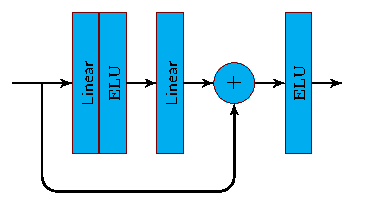
\includegraphics[scale = 1.25]{ResNet_Unit_MLP.pdf}};
			
			\draw[decorate sep={1mm}{2.5mm},fill] ($(RB2.east) + (0.15,0)$) -- ($(RB3.west) + (-0.05,0)$);		    
			\draw[thick, -latex] (Input) -- (WL1);
			\draw[thick, -latex] (WL1) -- (RB1);
			\draw[thick, -latex] (RB1) -- (RB2);
			\draw[thick, -latex] (RB3) -- (final);
			\draw[thick, -latex] (final) -- (Output);
			
			\draw[thick, dashed, latex-] (resnet_unit.south) +(-0.cm,-0.1cm) to[out=190,in=-30] (RB1.south);
			\draw[thick, dashed, latex-] (resnet_unit.north) +(0cm,0.1cm) to[out=170,in=30] (RB1.north);
			
			\node[below = 0cm of Input.south] ()  {$n\times 1$}; 
			\node[below = 0cm of WL1.south] ()  { $k\times 1$}; 
			\node[below = 0cm of RB1.south] ()  { $k{\times}1$}; 
			\node[below = 0cm of RB2.south] ()  { $k{\times}1$}; 
			\node[below = 0cm of RB3.south] ()  { $k{\times}1$}; 
			\node[below = 0cm of final.south] ()  { $k{\times}1$}; 
			\node[below = 0cm of Output.south] ()  { $n{\times}1$}; 
		\end{tikzpicture}
	\end{tabular}	
};
	\node[ fill = green!10!white,draw = green!50!black, text = black, thick,rounded corners = 0.5ex, above right =3cm and 0.2cm of MLP.west] (a) {\Huge (a)
	};
	\node[ fill = green!10!white,draw = green!50!black, text = black, thick,rounded corners = 0.5ex, above right =2.9cm and .2cm of Resnet_MLP.west] (b) {\Huge (b)
};

	\end{tikzpicture}
\end{document}
